\documentclass[11pt,a4paper]{scrartcl}
\usepackage[T1]{fontenc}
\usepackage[utf8]{inputenc}
\usepackage[ngerman]{babel}
\usepackage{microtype}
\usepackage{lmodern}
\usepackage{amsmath}
\usepackage{amsfonts}
\usepackage{amssymb}
\usepackage{enumerate}
\usepackage{graphicx}

\begin{document}

\author{Gruppe 14\\Max-Emanuel Hoffmann\\Ralf Vogler\\Sebastian Wiesner}
\title{Verteilte und Web-Informationssysteme}
\subtitle{Blatt 12}

\maketitle

\setcounter{section}{1}

\section{Benchmarking}

Tabelle~\ref{tab:results} zeigt die Ergebnisse des Benchmarks.
Abbildung~\ref{fig:tps} stellt die Transaktionen pro Sekunde verschiedener
Konfiguration da.

\begin{table}[h]
  \centering
  \begin{tabular}{l|r|r|r|r}
    \textbf{Anzahl OLAP-Prozesse} & \textbf{0} & \textbf{1} & \textbf{2} &
    \textbf{3} \\
    \hline
    TFork (in ms) & 0 & 0,343 & 0,312 & 0,425 \\
    TPS & 2743544 & 2295489 & 2121426 & 1172926 \\
    TQuery (in ms) & 0 & 36,99 & 53,025 & 73,316 \\
    TTrans (in ms) & 364,492 & 435,637 & 471,381 & 852,568 \\
  \end{tabular}
  \caption{Benchmark-Ergebnisse}
  \label{tab:results}
\end{table}

\begin{figure}[h]
  \centering
  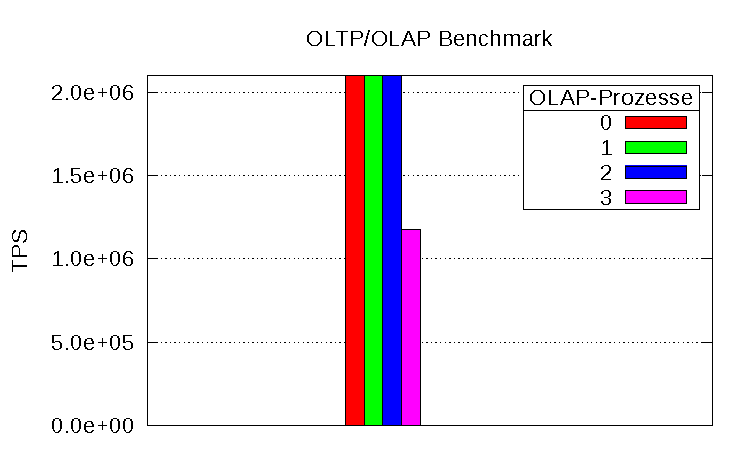
\includegraphics[scale=.75]{TPS.pdf}
  \caption{Transaktionen pro Sekunde}
  \label{fig:tps}
\end{figure}

Die Messungen wurden in einer virtuellen Maschine mit zwei Kernen zu je 3 Ghz
durchgeführt.  Detaillierte Informationen über die Prozessoren sind in der
beiliegenden Datei \texttt{results.txt} zu finden.  Das Programm wurde zur
Durchführung der Messungen mit \texttt{-DCMAKE\_BUILD\_TYPE=RelWithDebInfo}
konfiguriert.  Als Compiler wurde der \texttt{g++}-Compiler in Version 4.6
verwendet.

\end{document}
